
\documentclass{article}

% if you need to pass options to natbib, use, e.g.:
%     \PassOptionsToPackage{numbers, compress}{natbib}
% before loading neurips_2019

% ready for submission
 %\usepackage{neurips_2019}

% to compile a preprint version, e.g., for submission to arXiv, add add the
% [preprint] option:
%     \usepackage[preprint]{neurips_2019}

% to compile a camera-ready version, add the [final] option, e.g.:
\usepackage[final]{neurips_2019}

% to avoid loading the natbib package, add option nonatbib:
%     \usepackage[nonatbib]{neurips_2019}

\usepackage[utf8]{inputenc} % allow utf-8 input
\usepackage[T1]{fontenc}    % use 8-bit T1 fonts
\usepackage{hyperref}       % hyperlinks
\usepackage{url}            % simple URL typesetting
\usepackage{booktabs}       % professional-quality tables
\usepackage{amsfonts}       % blackboard math symbols
\usepackage{nicefrac}       % compact symbols for 1/2, etc.
\usepackage{microtype}      % microtypography
\usepackage[labelfont={bf}]{caption}
\usepackage{booktabs,lipsum}
\usepackage{graphicx}
\usepackage{subcaption}
\graphicspath{{./images/}}


\title{LIPS: Learning Inaudible Processed Speech}


\author{%
  John C. Merfeld \\
  Department of Computer Science\\
  Boston University\\
  Boston, MA 02215 \\
  \texttt{jcmerf@bu.edu} \\
	\And
  Allison Mann \\
  Department of Computer Science\\
  Boston University\\
  Boston, MA 02215 \\
  \texttt{ainezm@bu.edu} \\
}

\begin{document}
\maketitle

\begin{abstract}
While translating speech to text and back again has become a household technology over the past decade, many situations do not lend themselves to such audio translation. Automated lip reading provides an alternate avenue for translating speech to text. In this paper, we introduce 1) a video-processing pipeline that prepares raw video and text data for predictive modeling, 2) a deep-learning-based word classifier model on the processed data, and 3) evaluation of our model on several different vocabularies. All of this adds context to the still-burgeoning field of automated lip reading, suggesting questions for future study.
\end{abstract}

\section{Introduction}

Lip reading is the process of identifying spoken words purely from lip movement without any audio data. It is notoriously difficult, even for humans, but it plays a crucial role in human communication. This is highlighted by the McGurk Effect, where one phoneme's audio is transplanted on top of another phoneme's video, causing a third phoneme to be perceived [1]. Hearing-impaired people especially rely on this method to understand speech without audio. 

Even the most skilled lip readers are able to achieve an accuracy of around 30\% when identifying isolated words, however. They rely on context, body cues, and hand gestures to fill in the gaps [2]. Commonly, humans also use lip reading in cases where discreet communication is necessary or in noisy environments where audio signal is not available.

With recent machine learning advances, attention has been drawn to this problem due to its many practical applications. Lip reading has promising applications in assisting hearing-impaired people. With automated lip reading, video annotation and translation become possible. Lip reading also has applications in surveillance and analysis of forensic video.

In this paper, we propose \textit{Learning Inaudible Processed Speech} (LIPS), a method for lip reading via deep learning. Our method treats lip reading as a word classification problem. After extensive video processing, we use convolutional neural networks to exploit spatio-temporal features from input video data.

\section{Related work}

In recent years, there have been many advances in lip reading. Preceding work can be organized into two groups: classification systems and sequence prediction systems. 

\subsection{Classification Systems}

The majority of work done on this problem has been in the development of classification systems. The classification system approach performs classification over words or phonemes rather than full sentence sequence prediction. Ninomiya et.al. used Hidden Markov Models for classification of words or phonemes [3]. Sui et.al. approach the lip reading problem with Boltzmann Machines [4] and Chung et.al. propose a deep neural network framework for word classification. Their method can effectively learn and recognize hundreds of words [5]. Thabet et. al. propose novel video processing methods and show experimental results over multiple classifiers including Multi-Layer Perceptron, Naive Bayes, Support Vector Machine and Logistic Regression. Their results were very impressive with accuracy of 65\% over 5 distinct words [6].

\subsection{Sequence Prediction Systems}

Comparatively, much less work has been done on sequence prediction systems for lip reading. These systems aim to translate end-to-end sentences from visual data rather than single word classification. Notable work in this category was done by Graves et.al who use deep learning with recurrent networks for end-to-end speech recognition [7]. Their work, while not strictly lip reading, influenced following sequence prediction for lip reading such as the work of Assael et.al. with their system LipNet. LipNet uses convolutional neural networks to provide a distribution over sequences of phonemes and demonstrates high accuracy, especially with respect to distringuishing phonemes [8].

\section{Method}

Transforming video footage into a lip-reading prediction requires a significant processing pipeline. In this section, we discuss the training dataset, how it was prepared for modeling, and the overall architecture of our model.

\subsection{Data}

The Oxford-BBC Lip Reading Sentences 2 (LRS2) Dataset was selecting for training. Details of its creation can be found in [9]. A brief summary of the data will follow.

  \begin{figure}[h!]
 \centering
  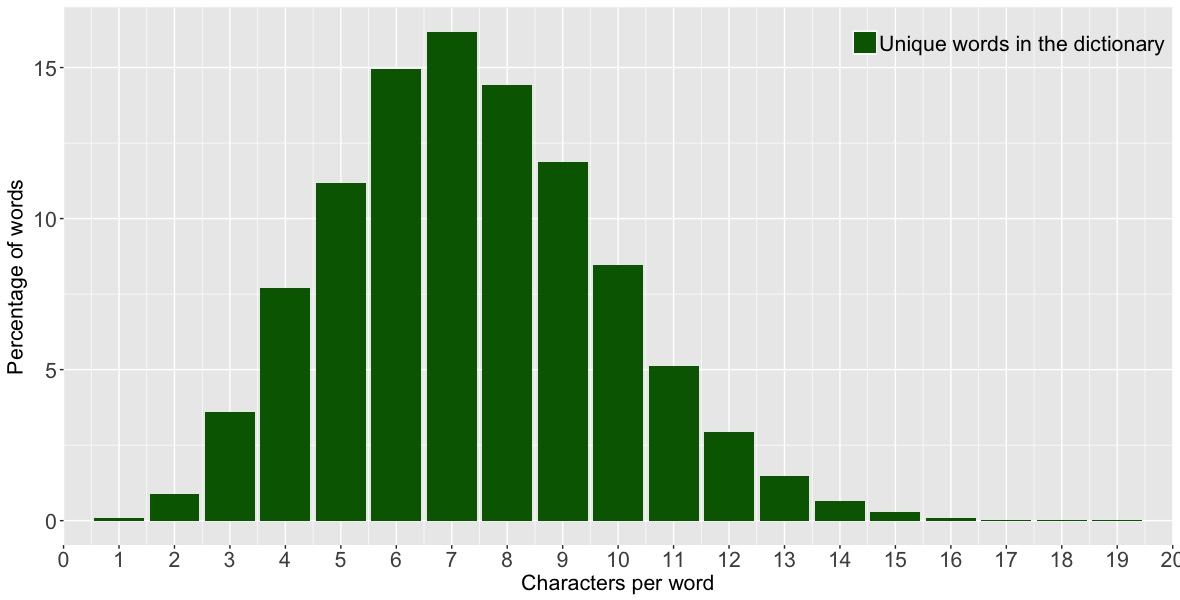
\includegraphics[width=0.8\textwidth]{uniqueWords}
 \caption{A dictionary $D$ containing an entry for each unique word in the dataset would have a modal character count of 7. Longer words tend to have more distinct visemes than shorter ones.}
 \end{figure}
 
The atomic units of raw data are video files, each around ten seconds long. The video clips come from BBC news and talk shows, but each frame's viewing window is shrunk to track the face of an individual speaker. A single speaker may span multiple clips, but LRS2 was designed specifically to include as many different faces as possible. Accompanying each video is a like-named metadata text file; this file contains an ordered list of words spoken in the clip along with timestamps indicating when the speaker starts and stops saying each word. These times are precise to the hundredth of a second.

   \begin{figure}[h!]
 \centering
  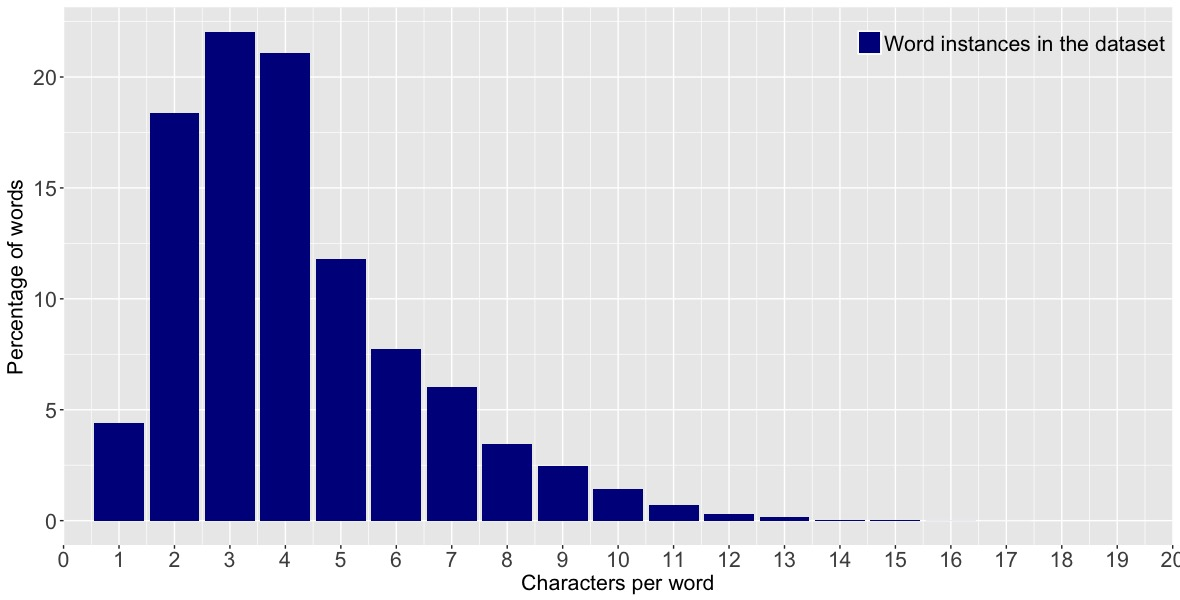
\includegraphics[width=0.8\textwidth]{wordInstances}
 \caption{Although there are more unique words with a higher character count, shorter ones appear much more often in the data.}
 \end{figure}


We did not use the entirety of LRS2; we limited our study to the "pre-train" segment because the "main" segment's text files do not include word timestamps. Still, the model's potential training examples encompassed over 2 million utterances of 41,427 unique words; 47GB of data in all.

\subsection{Feature Processing}

Consider an example pipeline whose output is a model that, given a video clip, predicts whether the speaker in that clip is saying the word "yes" or the word "no." So as to act within the realm of computational feasibility, we assign a parameter $N_{files}$ as an approximator for the size of this model's training set.

First, we prepare a dictionary mapping strings to unique integers. We formally define this as a set $D = \{\hbox{'YES'}: 0, \hbox{'NO'} : 1\}$ Next, $N_{files}$ text files are parsed word by word. If a word in the file is 'YES' or 'NO,' it is recorded, along with its beginning and ending timestamps.

Next, the videos corresponding to those $N_{files}$ text files are loaded and converted to greyscale. If a clip contains a word belonging to $D$, every frame between that word's two timestamps is recorded into its own 2D array of integers between 0 and 255. Thankfully, the videos in LRS2 are already of a uniform height and width, so no resizing is necessary. Together, this list of 2D arrays composes a 3D object we call a \textbf{word clip}. Note that at this stage, audio information is no longer present in the data representing the video.

Of course, each word instance may be composed of a different number of frames, depending on how long the speaker took to say the word. The model, however, will expect every input to be of the same dimension. Thus, we find the median length in frames of every word clip already created. If a word clip's frame count is higher than the median, it is evenly downsampled. Word clips that are too short have some of their frames repeated until they reach the median frame count. At the end of this preliminary process, then, we have a list of data objects pairing a word with a 3D word clip object of uniform size.

   \begin{figure}[h!]
 \centering
  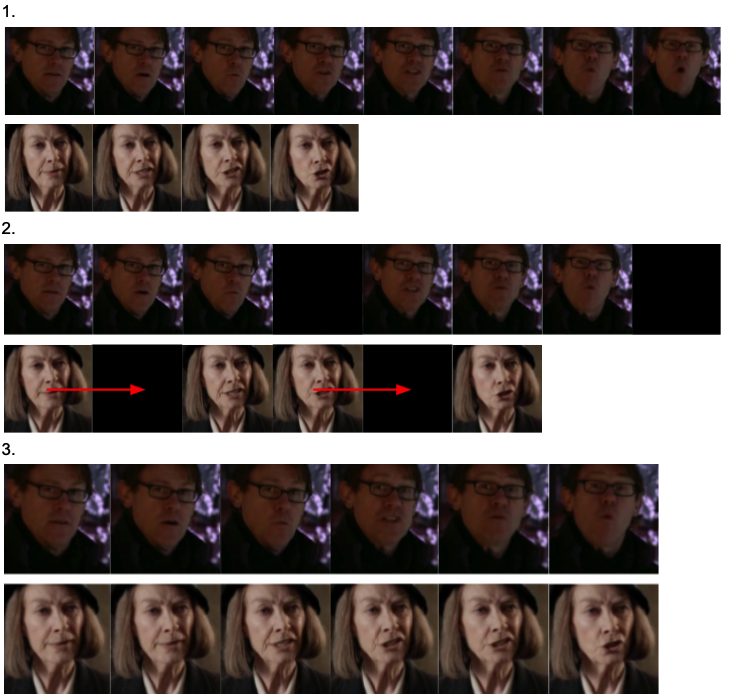
\includegraphics[width=0.8\textwidth]{sampling}
 \caption{In the above example, both clips must be resized to 6 frames. The first clip has frames removed at regular intervals, while the second clip has frames duplicated at regular intervals. The result is an input object of uniform size.}
 \end{figure}

Until now, we have dealt with word clips of the speaker's entire face. However, the model's task is far simpler if it only sees the speaker's mouth. We use dlib's face recognition library to detect facial features on each frame of each video. dlib is a C++ library that contains a toolkit of machine learning algorithms [10]. We primarily used "Shape Predictor 68 Face Landmarks" which extracts coordinates of 68 landmarks of the face. These landmarks represent points on the mouth, nose, eyes and so forth. We take a standard size bounding box centered around the mouth to crop each frame. 

This results in all frames being normalized to a standard size without affecting the aspect ratio. This method is reliable because our dataset contains video data centered around the face of the subject, and the videos were normalized in a previous step. This ensures that the face of the subject is roughly the same size in each video.

   \begin{figure}[h!]
 \centering
  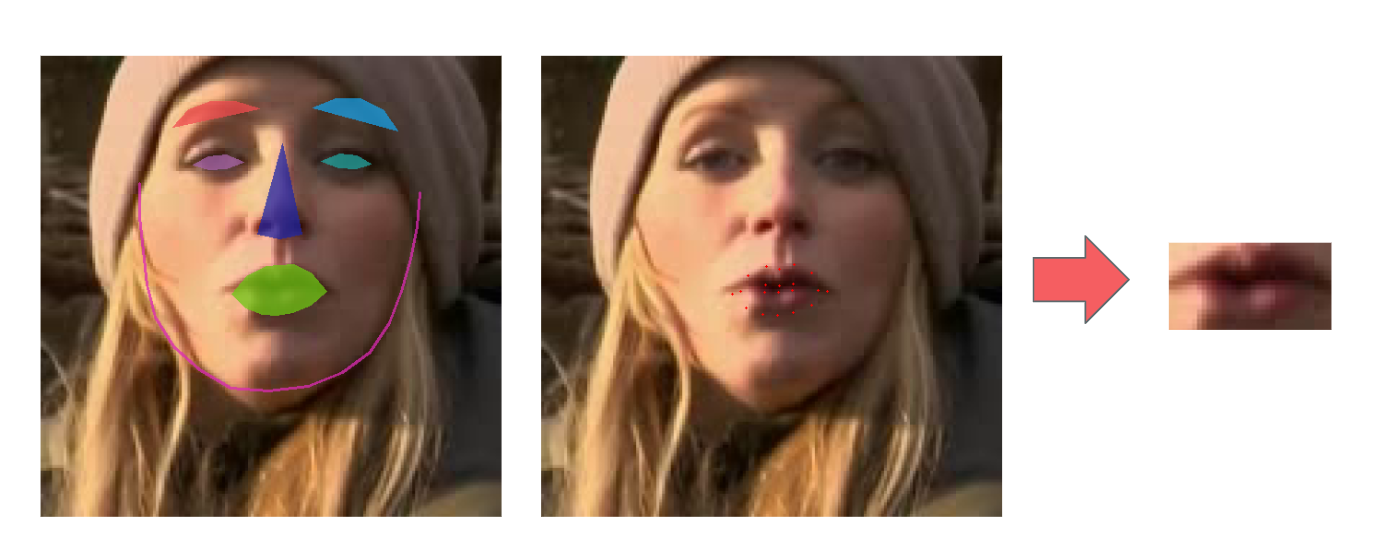
\includegraphics[width=0.8\textwidth]{dlib}
 \caption{We used dlib's face recognition library to detect and extract the speaker's mouth in each frame. dlib is able to detect coordinates of facial features as shown in the figure above. We take a bounding box around the points associated with the mouth for this project.}
 \end{figure}


Finally, we concatenate the frames of a video to make a long image. In the end, if each word is captured in $n$ cropped frames with dimension $h$ x $w$ then the resulting feature vector will have dimension $h$ x $nw$.

Thus, at the end of the pipeline, the model is prepared to be trained. To generalize this pipeline, we simply redefine $D$ to include whatever words the model needs to distinguish between. To train models quickly, we can reduce $N_{files}$ and temporarily store processed video data; to validate them, we can increase $N_{files}$ to include the entire training set.

\subsection{Model}

Once our video data has been processed, we create label vectors via one-hot encoding. If the total dictionary has $k$ words, then we create a vector of length $k$ where each entry is 0 except at one location where it is 1. Each cell represents a word in the dictionary, and a 1 in that cell signifies a label of the corresponding word.

The model we use is a convolutional neural network (CNN) because it exploits spatiotemporal features in the input image by performing stacked convolutions over the image. Our model has two convolutional layers each with reLU activation followed by max pooling. Finally, we have a global max pooling hidden layer to flatten the features and an output layer of size $k$. We take the softmax of the output to obtain probabilities of each word, and we use categorical cross entropy to train the model. For testing purposes, we assign the predicted word to be the word associated with the max entry of the output.

   \begin{figure}[h!]
 \centering
  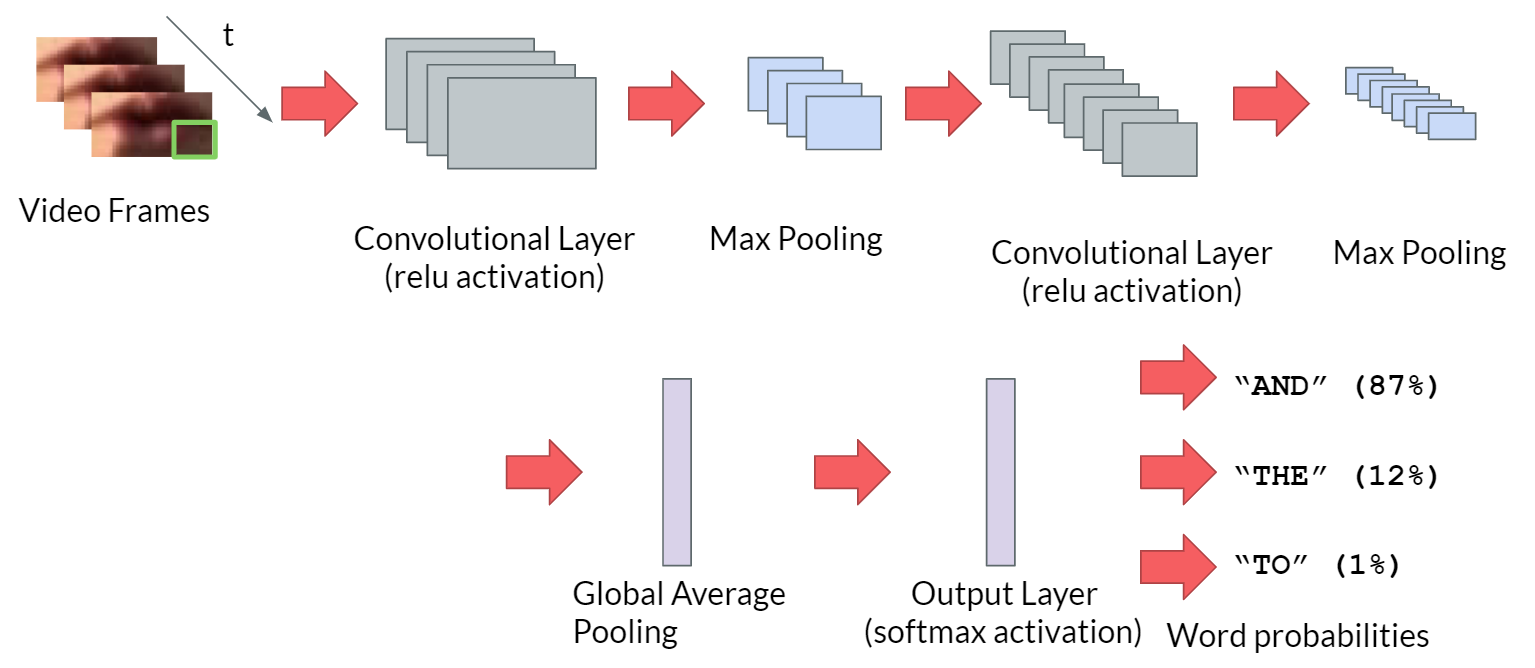
\includegraphics[width=0.8\textwidth]{model}
 \caption{The LIPS model architecture. A sequence of $n$ frames is used as input, and is processed by two convolutional layers followed by spatial max pooling.}
 \end{figure}

\section{Evaluation}

We performed multiple experiments over different dictionaries and sample sizes. We also experimented with hyper-parameters such as number of epochs, dropout, number of neurons on each layer of our model.

The experiments were conducted on Boston University's Shared Computing Cluster (SCC). For the flagship experiment on $D_{exp}$, described in Table 1, the pipeline process was run using $N_{files} = 10,000$, or about 11\% of the total data. Runs with a larger value for $N_{files}$ appeared to cause memory issues and were aborted by the cluster. 


\begin{table}[htbp]\centering
\def\sym#1{\ifmmode^{#1}\else\(^{#1}\)\fi}
\caption{$D_{exp}$ contains the words that the flagship models were trained to classify}
\begin{tabular}{l*{3}{c}}
\toprule
Word   &   Percentage of input set \\
\midrule
ABOUT            & 10.77\%  \\
BECAUSE                &   7.68\%   \\
GOING                &   8.40\%   \\
PEOPLE                &   6.26\%   \\
REALLY                &   7.15\%   \\
RIGHT                &   4.24\%   \\
SOMETHING               &   3.74\%   \\
THERE                &   8.58\%   \\
THINK                &   9.26\%   \\
THIS               &   19.33\%   \\
WHICH               &   6.58\%   \\
WOULD               &   8.01\%   \\
\bottomrule
\end{tabular}
\end{table}

\subsection{Results}

Our preliminary experiment was performed over a small dictionary, $D_{prelim}$ = \{"AND", "TO", "THE"\}, due to their prevalence in our dataset. We trained the CNN over 268 samples and tested over 54 samples, for a 80-20\% split. We were able to get very promising results with our model, with accuracy at 41\% with this experiment. 41\% accuracy is significantly better than random chance, at 33\%. The model primarily predicted "AND" because it was the most common word in the dataset, but we can see that it was able to classify "TO" fairly reliably, likely because this word has more distinctive visemes.

   \begin{figure}[h!]
 \centering
  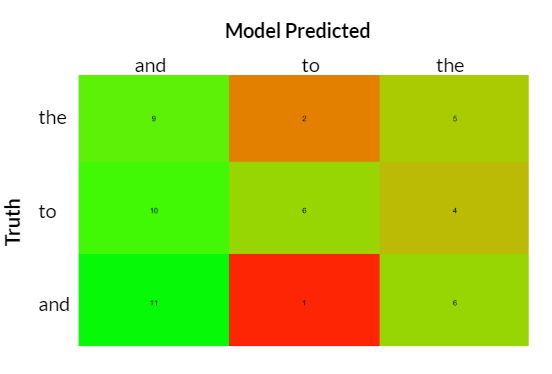
\includegraphics{result1}
 \caption{A confusion matrix for our preliminary result over a small sample dataset. LIPS achieves an accuracy of 41\%.}
 \end{figure}

We expanded our result to a larger dataset consisting of 12 words in a dictionary $D_{exp}$ (see Table 1). While the preliminary result is interesting, the words in $D_{exp}$ are longer and thus their videos contain more frames and visemes. This fact also increases the size of the input and output dimension of our model significantly. We trained over 1508 samples and tested over 377 samples.

With this experiment, we were able to obtain accuracy much higher than chance (8.33\%) at 21\% using 200 epochs and dropout of .05. We observe that it is able to classify "ABOUT", "WOULD", and "THIS" with some reliability compared to other words in this set. We also see some interesting phenomena, such as that "THIS" and "THINK" are commonly swapped by the model, which makes sense qualitatively given how similar they are.

   \begin{figure}[h!]
 \centering
  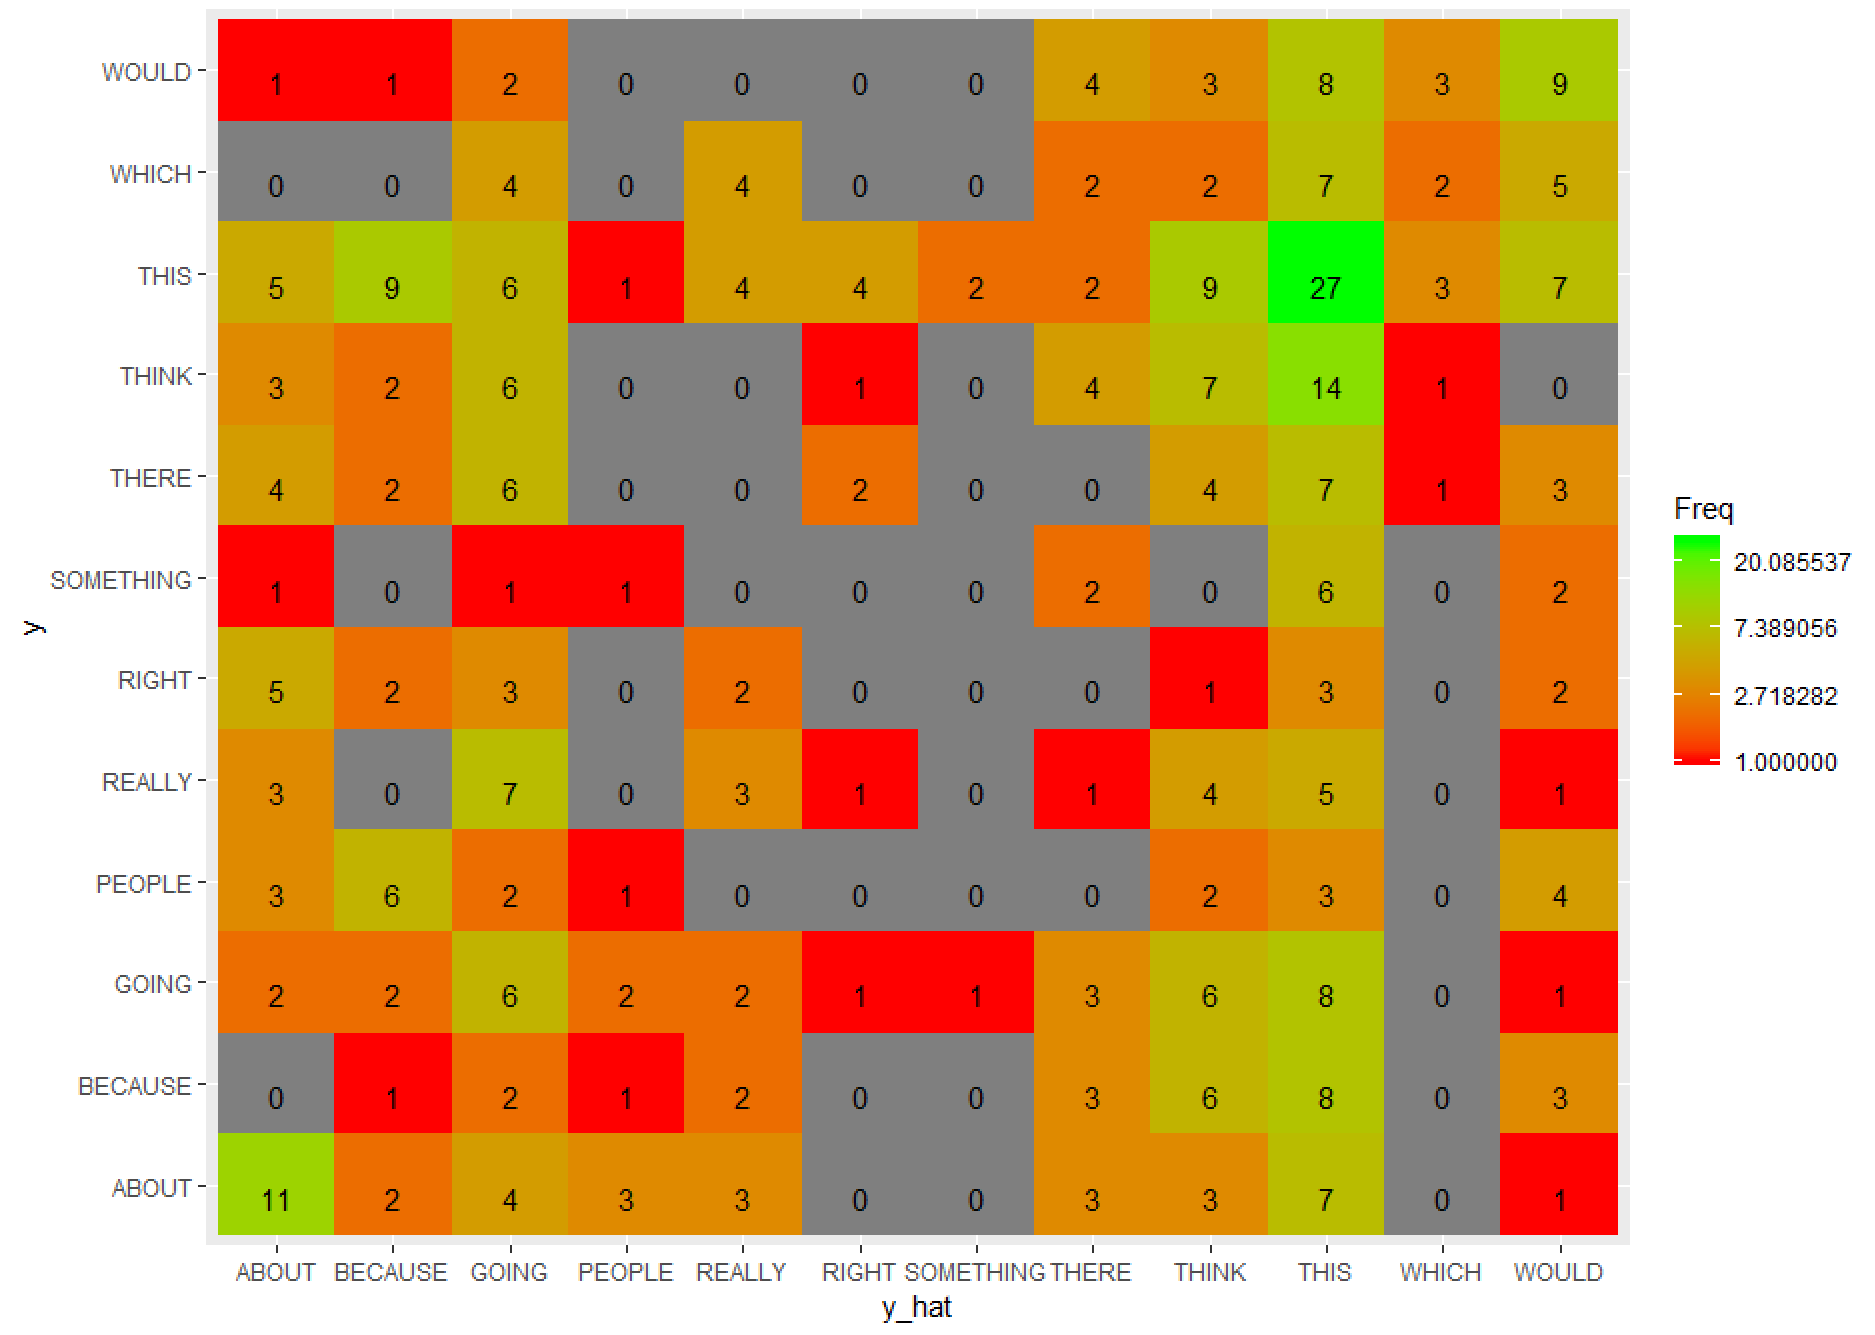
\includegraphics[width=0.8\textwidth]{result2}
 \caption{A confusion matrix for our result over a larger sample dataset. LIPS achieves an accuracy of 21\%.}
 \end{figure}

\subsection{Tuning hyperparameters}

Additionally, hyperparameter experiments were run on the same $D_{exp}, N_{files} = 10,000$ dataset. In one test, the number of training epochs was varied between 25 and 400. In another, the dropout rate was varied between 0.2 and 0.8. As Table 2 shows, these changes generally had no significant effect on the model's accuracy.

\begin{table}[!htb]
    \caption{For the most part, neither the amount of time spent training on $D_{exp}$ nor the number of nodes dropped from the network seemed to affect the model's performance on the test set}
    \begin{subtable}{.5\linewidth}
      \caption{}
      \centering
        \begin{tabular}{l*{3}{c}}
\toprule
Number of epochs   &   Model accuracy\\
\midrule
25           & 22.28\%  \\
50               &   21.48\%   \\
100                &   20.69\%   \\
200                &   22.02\%   \\
400                &   20.42\%   \\

\bottomrule
\end{tabular}
    \end{subtable}%
    \begin{subtable}{.5\linewidth}
      \centering
        \caption{}
        \begin{tabular}{l*{3}{c}}
\toprule
Dropout ratio  &   Model accruacy \\
\midrule
0.2           & 15.38\%  \\
0.3                &   20.42\%   \\
0.4                &   19.63\%   \\
0.5                &   19.63\%   \\
0.6                &   20.95\%   \\
0.7                &   21.48\%   \\
0.8               &   18.30\%   \\

\bottomrule
\end{tabular}
    \end{subtable} 
\end{table}

\section{Conclusion}

We proposed LIPS, a system to classify spoken words from processed video input using machine learning. We introduced a video-processing pipeline that uses face recognition software and segmented videos to produce input to our model as well as a convolutional neural network word classifier. We are able to achieve accuracy significantly higher than chance over several vocabularies, and performance will likely improve further with more data. 

Possible future work includes applying LIPS to larger datasets. Processing video data is expensive; it takes a lot of disk space and time. However, for performance of deep learning models, ideally we would process thousands of samples for each word.

\section*{References}
\small

[1] McGurk H. \ \& MacDonald J. \ (1976) Hearing lips and seeing voices. {\it Nature} {\bf 264} (5588): 746–8.

[2] Altieri, N. A.\ \& Pisoni, D. B. \ \& Townsend, J. T.\  (2011). Some normative data on lip-reading skills (L).{\it The Journal of the Acoustical Society of America}  {\bf 130} (1), 1–4.

[3]  Ninomiya, N. Kitaok\ \&, S. Tamura \ \& Y. Iribe \ \&  K. Takeda\ (2015) Integration of deep bottleneck features for audio-visual speech recognition. {\it In International Speech Communication Association}

[4] C. Sui \ \& M. Bennamoun \ \& R. Togneri (2015) Listening with Your Eyes: Towards a Practical Visual Speech Recognition System Using Deep Boltzmann Machines. {\it 2015 IEEE International Conference on Computer Vision (ICCV)} 154-162.

[5] J. S. Chung\ \& A. Zisserman\ (2016) Lip reading in the wild. {\it Asian Conference on Computer Vision} 87-103.

[6] Z. Thabet\ \& A. Nabih, K. Azmi\ \& Y. Samy \ \& G. Khoriba and M. Elshehaly \ (2018) Lipreading using a comparative machine learning approach. {\it 2018 First International Workshop on Deep and Representation Learning (IWDRL)} 19-25.

[7]  Graves \ \& N. Jaitly \ (2014) Towards end-to-end speech recognition with recurrent neural networks. {\it In International Conference on Machine Learning} 1764–1772

[8] Assael, Y.M\ \& Shillingford, B. \ \& Whiteson, S. \ \& Freitas, N.D. (2016). LipNet: Sentence-level Lipreading. {\it CoRR}

[9] T. Afouras\ \& J. S. Chung\ \& A. Senior\ \& O. Vinyals\ \& A. Zisserman \ (2018). Deep Audio-Visual Speech Recognition. {\it IEEE transactions on pattern analysis and machine intelligence.}

[10] R.-L. Hsu\ \& M. Abdel-Mottaleb\ \& A. K. Jain \ (2002) Face detection in color images. {\it IEEE transactions on pattern analysis and machine intelligence} {\bf 24} (5), 696-706.

\end{document}